\documentclass[a4paper]{scrartcl}
\usepackage{scrpage2}
\usepackage[ngerman]{babel}
\usepackage[T1]{fontenc}
\usepackage[utf8]{inputenc}
%\usepackage[pdftex]{graphicx}
%\usepackage[intlimits]{amsmath}
%\usepackage{listings}
%\lstset{frame=single,breaklines=true}
\usepackage{ amssymb }
\usepackage{amsmath}
\usepackage{hyperref}
\usepackage{enumerate}
\usepackage[a4paper, total={19cm, 23cm}]{geometry}
\usepackage{stmaryrd}
\usepackage{esvect}
\usepackage{graphicx}
\pagestyle{scrheadings}
\pagenumbering{gobble}
\ihead{Übungsblatt 4\\Nils Werner 108012219293}
\chead{\\Paul Rösler 108012225686	}
\ohead{Übungsgruppe: Mo. 16:00\\Daniel Teuchert 108012214552}
\setheadsepline{0.4pt}
\begin{document}

\section*{Aufgabe 1}
\begin{figure}[htp] \centering{
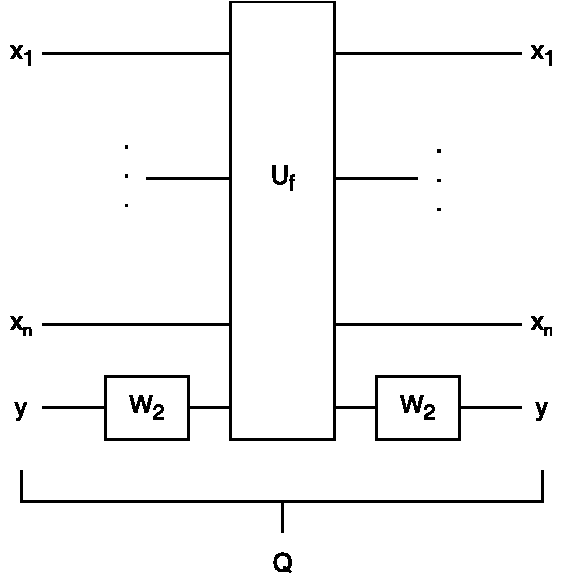
\includegraphics[scale=0.5]{ue4a1q.pdf}}
\caption{Quantenschaltkreis Q entspricht dem Schaltkreis aus Präsenzübung 4 Aufgabe 4}
\label{p4a4}
\end{figure}
Gesucht ist ein Schaltkreis, welcher die reversieble Einbettung $U_f$ $|\vv{x}y\rangle \xrightarrow{} |\vv{x}\rangle \bigotimes |f(\vv{x}) \oplus y \rangle$ berechnet.
Ein Bestandteil des Schaltkreises darf das Quantengate Q sein, welches dem Schaltkreis aus Aufgabe 4 der Präsenzübung 4 entspricht (Abb. \ref{p4a4}).
Das $U_f$ dieser Aufgabe entspricht dabei dem $U_f$ der Präsenzaufgabe.
Um nun aus Q das Gate $U_f$ zu erhalten muss jeweils die Auswirkung des Gates $W_2$ auf $|y\rangle$ ausgeglichen werden. Dazu kann man die Eigenschaft von $W_2$ nutzen, dass $|y\rangle \xrightarrow{W_2} \xrightarrow{W_2} |y\rangle$ ist.
\begin{figure}[htp] \centering{
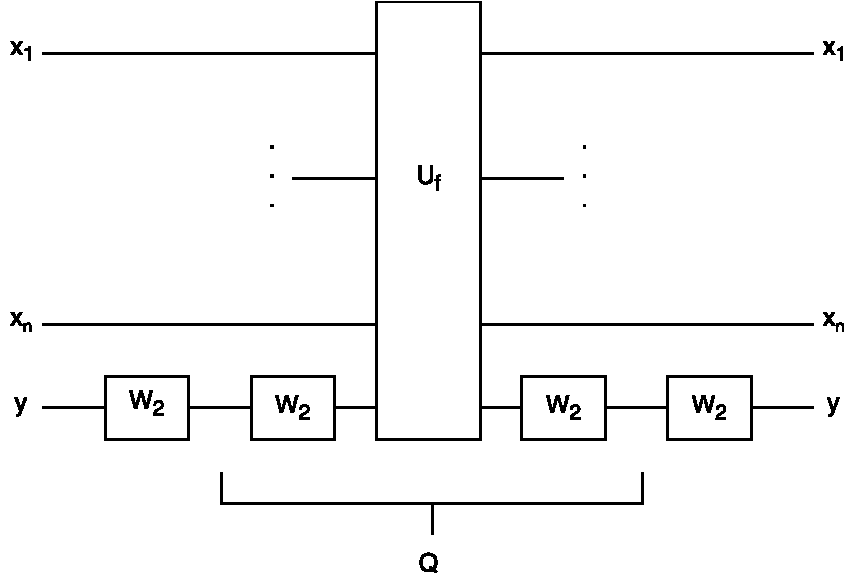
\includegraphics[scale=0.5]{ue4a1q2.pdf}}
\caption{Schaltkreis aus $W_2$ und Q um $U_f$ zu selektieren}
\end{figure}\\
Das voran und nachstellen von $W_2$ auf $|y\rangle$ sorgt nun dafür, dass auf $|\vv{x}y\rangle$ nur $U_f$ wirkt und das der gesuchten Schaltung entspricht.

\newpage
\section*{Aufgabe 2}
\begin{enumerate}[a)]
\item ~\\
\begin{figure}[htp] \centering{
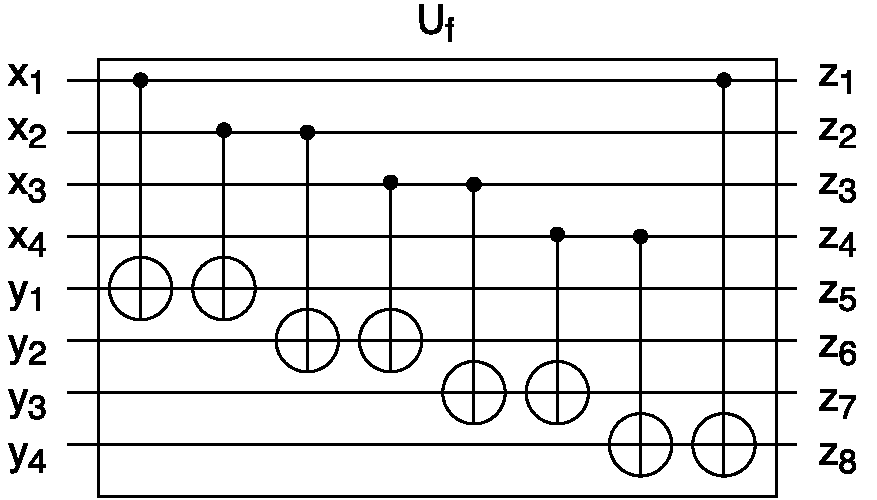
\includegraphics[scale=0.5]{ue4a2a.pdf}}
\caption{Quantenschaltkreis für die reversible Einbettung von $f$}
\end{figure}

\item ~\\
\begin{figure}[htp] \centering{
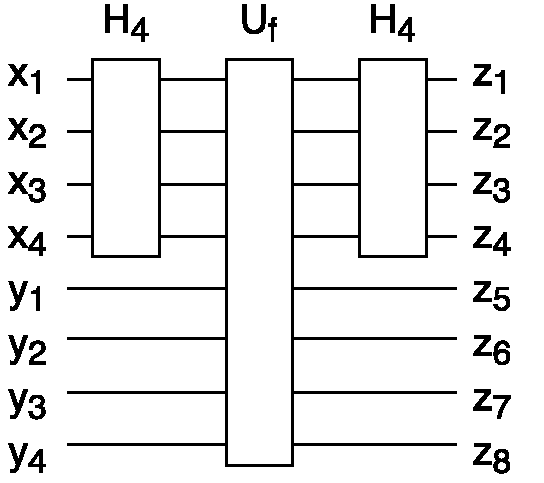
\includegraphics[scale=0.5]{ue4a2b.pdf}}
\caption{Quantenschaltkreis $Q_S$ des Algorithmus von Simon für dieses $f$}
\end{figure}

\item

$ \begin{pmatrix}
1 & 1 & 0 & 0 \\
1 & 0 & 1 & 0 \\
1 & 0 & 0 & 1 \\
0 & 0 & 0 & 0 \\
\end{pmatrix} \begin{pmatrix}
s_1 \\
s_2 \\
s_3 \\
s_4 \\
\end{pmatrix} = \begin{pmatrix}
0 \\
0 \\
0 \\
0 \\
\end{pmatrix} \Leftrightarrow \begin{pmatrix}
s_1 \\
s_1 \\
s_1 \\
0 \\
\end{pmatrix} = \begin{pmatrix}
s_2 \\
s_3 \\
s_4 \\
0 \\
\end{pmatrix}$ \\
$\Rightarrow (s_1, s_2, s_3, s_4) = (1, 1, 1, 1) \vee (s_1, s_2, s_3, s_4) = (0, 0, 0, 0)$
\item $Pr[n-1$ Vektoren aus $\mathbb{F}_2^n$ sind linear unabhängig$] $\\
$=\prod_{i=1}^{n-1} Pr[y_{i}\neq 0^n \wedge y_{i}$ ist l.u. von $y_1$ bis $y_{i-1}]$\\
$=\prod_{i=0}^{n-2} Pr[y_{i+1}\neq 0^n \wedge y_{i+1}$ ist l.u. von $y_1$ bis $y_i]$\\
$=\prod_{i=0}^{n-2} Pr[y_{i+1}\neq 0^n \wedge y_{i+1} \notin \{y_1,..,y_i\} \wedge y_{i+1}$ ist nicht Summe zweier oder mehr ungleicher Summanden aus $\{y_1,..,y_i\}]$\\
$=\prod_{i=0}^{n-2} \frac{2^n-1-i-{i \choose 2}-{i \choose 3}-..-{i \choose i}}{2^n} =\prod_{i=0}^{n-2} \frac{2^n - \sum_{j=0}^i{i \choose j}}{2^n} = \prod_{i=0}^{n-2} \frac{2^n - 2^i}{2^n}= \prod_{i=0}^{n-2} (\frac{2^n}{2^n}-\frac{2^i}{2^n})= \prod_{i=0}^{n-2} (1-2^{i-n})$\\

$\prod_{i=0}^{2}(1-2^{i-4}) = (1-2^{-4})(1-2^{-3})(1-2^{-2})=\frac{315}{512}\approx 62 \%$
\end{enumerate}

\newpage
\section*{Aufgabe 3}
Da $S_u=\{\wedge, \neg, c\}$ universell ist, kann insbesondere jede reversible Funktion mittels $S_u$ dargestellt werden. Es genügt daher, jedes Element als Verknüpfung von $T$, Hilfsvariablen und $0$, $1$ zu
schreiben (s. Script).\\
Sei $S_q' = \{T_{\wedge},T_{\neg},T_{c}\}$ das r-reversible Pendant zu $S_u$ mit dem gezeigt wird, dass $S_q = \{T\}$ r-reversibel ist.\\
$T_{\wedge} = T(x_1,x_2,0) = (x_1,x_2,x_1x_2)$\\
$T_{\neg} = T(x_1,1,1) = (x_1,1,1+x_1) = (x_1,1,-x_1)$\\
$T_{c} = T(x_1,1,0) = (x_1,1,x_1)$\\
$S_u=\{\wedge, \neg, c\}$ kann also durch $S_q' = \{T_{\wedge},T_{\neg},T_{c}\}$ dargestellt werden, wobei lediglich das Toffoli-Gate $T$ und $0$, $1$ verwendet werden. Daraus folgt, dass $S_q = \{T\}$ r-reversibel ist.


\newpage
\section*{Aufgabe 4}
\begin{enumerate}[a)]
\item Nach dem Satz von Lagrange gilt: Die Ordnung jeder Untergruppe teilt die Ordnung der Gruppe.\\
Da $<a>$ in $\mathbb{Z}_{p_i}^*$ eine Untergruppe der Gruppe $<a>$ in $\mathbb{Z}_N^*$ mit $a$ ist Generator ist, folgt $t_i | t$.\\
Daraus folgt, dass $t\geq kgV(t_1,..,t_k)$


\item $s_i = r_i$ gilt gdw. $a$ ein quadratischer Rest modulo $p_i$ ist.\\
 Da $a$ uniform aus $\mathbb{Z}_N^*$ gezogen wird, gilt für jedes $i$ unabhängig: $a\in_R\mathbb{Z}_{p_i}^*$\\
Ausserdem gilt für $\mathbb{QR}=\{x\in \mathbb{Z}_{p_i}^*|x$ ist Quadratischer Rest modulo $p_i\}$: $|\mathbb{QR}|=\frac{|\mathbb{Z}_N^*|}{2}$. Dies liegt daran, dass $x \rightarrow x^2$ eine $2$ zu $1$ Abbildung ist ($x^2=(-x)^2$).\\
Somit gilt Ws[$a$ ist quadratischer Rest modulo $p_i$]$=\frac{1}{2}$, $\forall a\in_R\mathbb{Z}_N^*$

\item 

\item $a^{2^{s-1}u}= a^{\frac{2^{s}u}{2}}$ mod $p_i$\\
Es gilt: ord$_{\mathbb{Z}_N^*}(a)=t=2^{s}u$ und ord$_{\mathbb{Z}_{p_i}^*}(a)=t_i=2^{s_i}u_i$\\
Wie in a) gezeigt, gilt $t=$ kgV$(t_1,...,t_k)$ und somit auch $s=$ max$\{s_1, ...,s_k\}$\\
Daraus folgt, das $u_i$ $u$ teilt, denn $t_i$ teilt $t$\\
$\Rightarrow u_i \cdot K = u$ für $K$ ungerade\\
$\Rightarrow a^{\frac{2^{s_i}u_i\cdot K}{2}}$ mod $p_i$ Es gilt: $t_i = $ ord$(a)$ mod $p_i$:\\
$\Rightarrow 1^{\frac{K}{2}} = 1^{\frac{1}{2}}$ mod $p_i$ Hierfür gibt es nur 2 Lösungen: $1$ und $-1$\\
In diesem Fall bleibt jedoch nur die Lösung $a^{2^{s-1}u}= -1$ mod $p_i$, da $a^{\frac{2^{s_i-1}u_i}{2}}$ nicht 1 sein kann, da $\frac{2^{s_i-1}u_i}{2} < t_i =$ ord$(a)$ mod $p_i$ 

\item Wie bereits in d) gezeigt, gilt: $a^{2^{s_i-1}u}$ mod $ p_i=-1$, falls $s_i\geq 1$\\
Fall 1: $s_i=s$\\
$\Rightarrow a^{2^{s-1}u} = a^{2^{s_i-1}u}=-1$ mod $p_i$\\
$\Rightarrow a^{2^{s-1}u} = -1$ mod $p_i$, falls $s_i=s$\\\\

Fall 2: $s_i < s \Rightarrow s = s_i+k$, mit $k\geq 1$\\
$\Rightarrow a^{2^{s-1}u} = a^{2^{s_i+k-1}u}=a^{2^{s_i-1}2^ku} = (a^{2^{s_i-1}u})^{2^k} = (-1)^{2^k} = 1^{2^{k-1}}= 1$ mod $p_i$\\
$\Rightarrow a^{2^{s-1}u} = 1$ mod $p_i$, falls $s_i<s$. Daraus folgt auch: $u_i$ teilt $u$, da beide Zahlen ungerade sind und somit nicht in $2^{s_i}$ bzw. $2^s$ enthalten sind.\\



\item
Falls gilt: $a^{2^{s-1}u}$ mod $p_i=-1 \Rightarrow a^{2^{s-1}u}+1=K\cdot p_i$, für ein $K\in \mathbb{Z}$\\
Fall 1: ggt$(N,K)=1$\\
$\Rightarrow$ ggt$(N, a^{2^{s-1}u}+1) = p_i$, also ein nicht-trivialer Teiler von $N$.\\\\

Fall 2: ggt$(N, K)=q$, aber $p_i$ teilt nicht $K$\\

$\Rightarrow$ ggt$(N, a^{2^{s-1}u}+1) = p_i \cdot q$, also ein nicht-trivialer Teiler von $N$. \\\\
 
Fall 3:  ggt$(N,K)=q$ und $p_i$ teilt $K \Rightarrow p_i$ teilt $q$ \\
$\Rightarrow$ ggt$(N, a^{2^{s-1}u}+1) = q$, also ein nicht-trivialer Teiler von $N$. \\\\

$\Rightarrow$ wenn $\exists i$, mit $a^{2^{s-1}u}$ mod $p_i=-1$, gilt ggt$(N, a^{2^{s-1}u})$ ist ein nicht-trivialer Teiler.\\
Dieser Fall tritt genau dann ein, wenn es ein $j$ gibt mit $s_j\geq 1$, denn dann gibt es ein $i$ mit $s_i=$ max$\{s_1, ..., s_k\}=s\geq 1$ und es gilt $a^{2^{s_i-1}u} =-1 = a^{2^{s-1}u}$ mod $p_i$.
Ws[$ s\geq 1$]$=$Ws[$\exists i \neq j$ mit $s_i \neq s_j$]$\geq\frac{1}{4}$ (siehe c))\\
$\Rightarrow$ Mit Ws $\frac{1}{4}$ ist ggt$(N, a^{2^{s-1}u})$ ein nicht-trivialer Teiler.



\item
Algorithmus:\\
\begin{enumerate}[1.]
\item Wähle $a\in_R \mathbb{Z}_N^*$ uniform
\item Berechne \texttt{PERIODE}($N,a$) und erhalte so $t =$ ord$_{\mathbb{Z}_N^*}(a)$ mit $t=2^s\cdot u$
\item Berechne $\frac{a^t}{a^2}+1=x$
\item Berechne ggT($N, x$)$=p$
\item Falls gilt: $p | N$ gebe $p$ aus, sonst gehe zu Schritt 1
\end{enumerate}

Korrektheit:
$x=\frac{a^t}{a}+1= \frac{a^{2^s\cdot u}}{a^2}+1= a^{2^{s-1}\cdot u}+1$\\
Es gilt mit Ws $\geq \frac{1}{4}$ dass ggT($N, x$)$=p$ ein nicht-trivialer Teiler von $N$ ist und das somit gilt $p|N$
Bei dem zweifachen durchlaufen von den Schritten 1-4 ist die Wahrscheinlichkeit einen nicht-trivialen Teiler gefunden zu haben schon bei $1-(\frac{3}{4})^2=0,4375=43,75 \%$

Laufzeit:



\end{enumerate}


\end{document}
